%Standard Header
\documentclass[10pt,a4paper,toc=listof,toc=bibliography]{scrartcl}
\usepackage[utf8]{inputenc}
\usepackage[ngerman]{babel}
\usepackage[T1]{fontenc}
\usepackage{amsmath}
\usepackage{amsfonts}
\usepackage{amssymb}
\usepackage[pdftex]{graphicx}

%\usepackage{epstopdf}                            %import .eps (from MATLAB)
\usepackage{geometry}
\geometry{left = 25mm, top = 25mm, right = 25mm, bottom = 25mm}
\usepackage{multirow}
\usepackage{pdfpages}                            %import pdf
\usepackage{textcomp}                            %degree celsius etc
\usepackage{gensymb}
\usepackage[hidelinks]{hyperref}                 %hidelinks removes red boxes from pdf
\usepackage[style=german, german=quotes]{csquotes}
\usepackage[backend=biber, style=numeric, citestyle=numeric, sorting=none]{biblatex}
\usepackage{float}

\usepackage[all,defaultlines=2]{nowidow}		%prevent Witwen and Schusterjungen
\usepackage{microtype}

\usepackage{color}
\usepackage{listings}                            %einbinden von Sourcecode

\usepackage{chemfig}
\usepackage{upgreek}
\usepackage{chemmacros}
\usepackage{chemformula}

\addbibresource{../DATA/bibresource.bib}        %Standardpfad für .bib Datei des Projektes

\usepackage{lmodern}

%\KOMAoption{DIV}{12}

%%%% alte Definition:
%% \DeclareMathSymbol{,}{\mathpunct}{letters}{"3B}
%%%% neue Definition:
%%\DeclareMathSymbol{,}{\mathord}{letters}{"3B}       %removes space in mathmode
\DeclareMathSymbol{*}{\mathbin}{symbols}{"01}

\newcommand{\mlab}{MATLAB}
%\renewcommand{\figurename}{Abb.}    %for article/report and non KOMA-Classes
\renewcaptionname{ngerman}{\figurename}{Abb.}

\setlength{\parindent}{0pt}          %keine Einschübe bei neuem Absatz

\addtokomafont{disposition}{\rmfamily} % serifes in headings

%SI-Units and correct spacing according to ISO-31
\usepackage[range-phrase = \ldots~]{siunitx}
\sisetup{locale=DE}
\sisetup{inter-unit-product=\ensuremath{{}*{}}}
\sisetup{per-mode=symbol}
%Listings environment for sourcecode
%\renewcommand{\lstlistlistingname}{Sourcecode}     %name in listof"sourcecode"
%\renewcommand{\lstlistingname}{Code}            %captionPreName

\lstset{breaklines}
\lstset{numbers=left}
\lstset{frame=single}
%\lstset{language=Matlab}
\lstset{showstringspaces=false}
\lstset{ %
	backgroundcolor=\color{white},   % choose the background color
	basicstyle=\footnotesize,        % size of fonts used for the code
	breaklines=true,                 % automatic line breaking only at whitespace
	captionpos=b,                    % sets the caption-position to bottom
	commentstyle=\color{olive},      % comment style
	escapeinside={\%*}{*)},          % if you want to add LaTeX within your code
	keywordstyle=\color{blue},       % keyword style
	stringstyle=\color{magenta},     % string literal style
	extendedchars=true,
	literate={ä}{{\''a}}1 {ö}{{\''o}}1 {ü}{{\''u}}1 {ß}{{\ss}}1,
	inputencoding=utf8,
}

% Site-Header with KOMA
%\usepackage[headsepline]{scrlayer-scrpage}    %headsepline makes line under header
%\ihead{}        %Inner-Head
%\ohead{}                    %Outer-Head
%\pagestyle{scrheadings}                        %activate Headings
%\setkomafont{pageheadfoot}{\normalsize}        %normal fontsize for headline

\renewcommand{\mkbegdispquote}[2]{\glqq}
\renewcommand{\mkenddispquote}[2]{\grqq#2}
\renewcommand{\mkcitation}[1]{ \textsuperscript{[}#1\textsuperscript{]}}  

\hyphenation{}
\hyphenation{}

\begin{document}
\begin{titlepage}
	
	\begin{figure}[H]
		\begin{minipage}{0.5\textwidth}
			\centering
			
\includegraphics[width=0.8\textwidth]{../DATA/Logo_Uni-Kassel.pdf}
			%\caption{Kugel mit Stativ}
			%\label{fig3}
		\end{minipage}\hfill
		\begin{minipage}{0.5\textwidth}
			\centering
			
\includegraphics[width=0.8\textwidth]{../DATA/Logo_solar.png}
			%\caption{Druckmessbohrung Kugel}
			%\label{fig4}
		\end{minipage}
	\end{figure}
	
		\vspace{3cm}
	
	\centering
	{\scshape\LARGE Praktikum Thermische Messtechnik \par}   %Title
	\vspace{1cm}
	{\scshape\Large Teil 1: Temperaturmessung \par}
	\vspace{1.5cm}
%	{\huge\bfseries  \par}  %Hauptüberschrift
	\vspace{2cm}
	{\Large Lena Völlinger \& Marvin Grosch\par}
	\vfill
	
	% Bottom of the page
	\begin{large}
		\begin{tabular}{l l}
			
			Praktikumstag: & 04.09.2020 \\
			Erstabgabe: & 05.10.2020\\
			Betreuer: & Markus Rusack \& Christoph Schmelzer\\
			Studiengang: & Master $\text{re}^2$\\
			Semester: & SoSe 2020\\
			Matrikelnr.: & 35597894, 35598242\\ 
		\end{tabular}
	\end{large}

\end{titlepage}

\pagenumbering{Roman}

\newpage
\tableofcontents
\listoffigures
\newpage

\pagenumbering{arabic}

\section{Einleitung}

Für den Versuch Temperaturmessung sollten verschiedene Temperatursensoren (Pt100 2L, Pt1000 2L, KTY 2L, NTC 2L) und ein Thermoelement Typ K an einem Metallblockkalibrator mit einem Pt-100 4L Referenzfühler, der zuvor an einer Wassertripelpunktzelle kalibriert wurde,  gemessen und deren Genauigkeit beurteilt werden. 
Die verschiedenen Temperaturensensoren wurden anhand von Fixpunkt- und Vergleichsmethode charakterisiert. 

Anschließend wurden Widerstandssensoren unterschiedlichen Typs mit einem Mulitmeter untersucht und Anhand ihrer Kennliniendiagramme identifiziert. 

Im dritten Teil wurde sich mit der berührungslosen Temperaturmessung befasst. Es erfolgte die Untersuchung verschiedener Materialien in einem temperierten Wasserbad mithilfe einer Wärmebildkamera. Dabei wurden die Unterschiede der Materialien und ihren Einfluss auf die Messung untersucht und analysiert. 
%\newpage
\section{Versuchsauswertung}

\subsection{Teil I: Kalibrierung}

\subsubsection{Fixpunktkalibrations an der Wassertripelpunktzelle}

Zunächst wurde der Pt-100 (Vierleiterschaltung) Referenzsensor anhand der Wassertripelzelle (Tripelpunkt bei \SI{0,01}{\celsius} und \SI{6,1}{\milli\bar}) mittels Fixpunktkalibration kalibriert. In der folgenden Abbildung \ref{fig:Fixpunkt} wird der Temperaturverlauf in Abhängigkeit der Zeit (die Scanrate beträgt \SI{1}{\sec}) für den Pt-100 Sensor abgebildet. 

\begin{figure}[H]
	\centering
	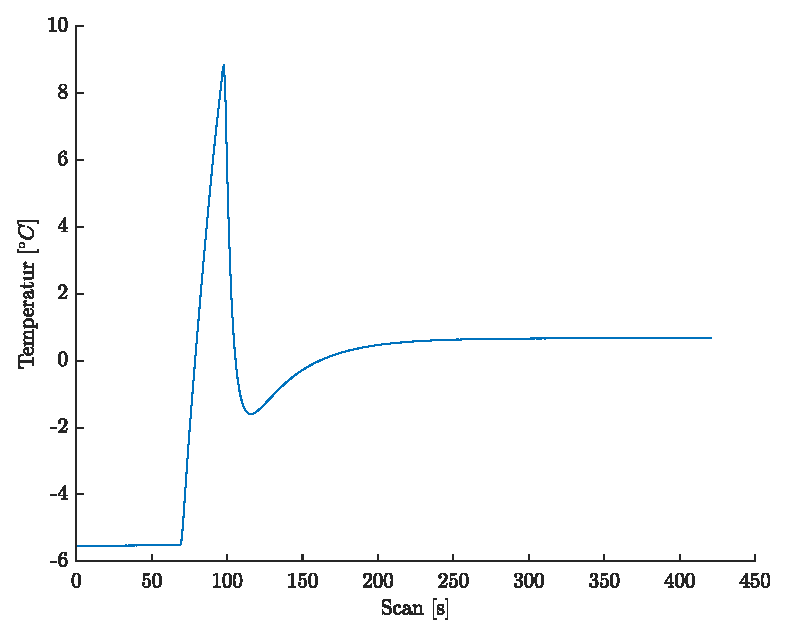
\includegraphics[height=0.3\textheight]{../MLAB/Fixpunktkalibration.eps}
	\caption[Temperaturverlauf des Pt100 Temperatursensors mittels Wassertripelpunktzelle]{ Temperaturverlauf des Pt100 Temperatursensors mittels Wassertripelpunktzelle im Metallblockkalibrator.}
	\label{fig:Fixpunkt}
\end{figure}

Folgende Daten wurden für den Mittelwert, die Standardabweichung und den Offset des Referenzsensors gegenüber der Temperatur der Tripelpunktzelle ermittelt: 


\begin{table}[H]
	\centering
	\caption{Mittelwert, Standardabweichung und Offset des Pt100 4L Referenzsensors zur Tripelpunktzelle.}
	\label{tab:VergleichTPZ}
	\begin{tabular}{cccc}
		Temperatur TP [\si{\celsius}] & avg & std & Offset \\ 
		\hline 
		\num{0.01} & \num{0.6691} & \num{0.0024} &  \num{0.6591}\\ 
	\end{tabular} 
\end{table}


Im folgenden wurden mit dem ermittelten Offset des Referenzsensors dessen Messwert korrigiert und bei den folgenden Berechnungen berücksichtigt und angepasst. 

\subsubsection{Vergleichskalibration der Sensoren}

Die Vergleichskalibration der unterschiedlichen Sensoren erfolgte in einem Temperaturbereich von \SI{0}{\celsius} bis \SI{80}{\celsius}, für die Messungen wurden über den Pt100 4L die Temperaturen \SI{0}{\celsius}, \SI{20}{\celsius}, \SI{40}{\celsius} und \SI{80}{\celsius} ausgewählt und über den Metallblockkalibrator eingestellt. In der folgenden Abbildung \ref{fig:Widerstand} sind die Widerstände der einzelnen Temperatursensoren gegen die ausgewählten Temperaturmesspunkt aufgetragen. 

\begin{figure}[H]
	\centering
	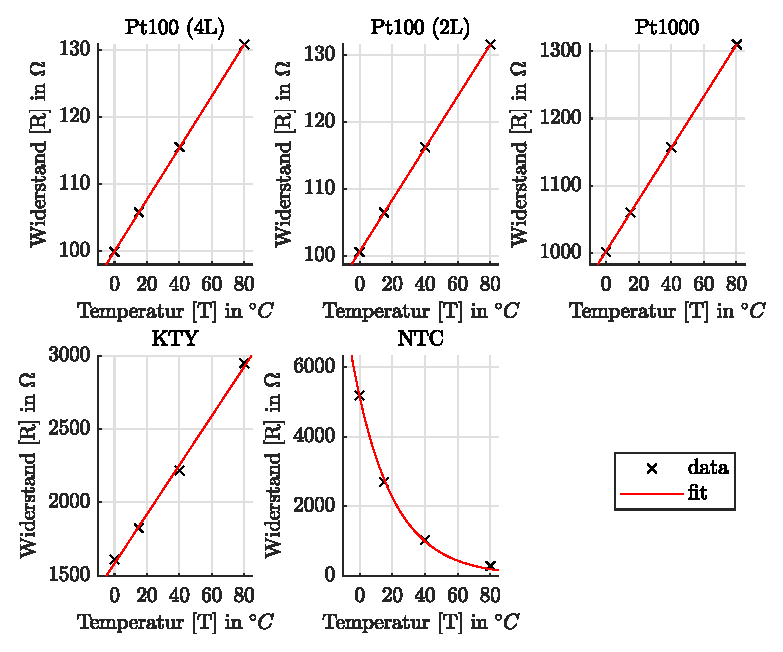
\includegraphics[height=0.5\textheight]{../MLAB/Widerstandsgeraden.eps}
	\caption[Ermittelte Widerstandswerte der untersuchten Temperatursensoren ]{Ermittelte Widerstandswerte der untersuchten Temperatursensoren (Pt100 4L, Pt100 2L, Pt1000, KTY, NTC bei den Temperturen \SI{0}{\celsius}, \SI{20}{\celsius}, \SI{40}{\celsius} und \SI{80}{\celsius} im Metallblockkalibrator eingestellt über den Pt100 4L Referenzsensor. }
	\label{fig:Widerstand}
\end{figure}

\begin{table}[H]
	\centering
	\caption{Fitfunktionen der Temperatursensoren.}
	\label{tab:FitFun}
	\begin{tabular}{ccS[separate-uncertainty,table-figures-uncertainty = 1]S[separate-uncertainty,table-figures-uncertainty = 1]S}
		
		Sensortyp & Regressionsfunktion & {Koeff $a$} & {Koeff $b$} & {$R^2$} \\
		
		Pt100 (4L) & $ax+b$ & 0.3849(48) & 99.9695(2168) & 1 \\
		Pt100 (2L) & $ax+b$ & 0.3864(49) & 100.62(22) & 1 \\
		Pt1000 & $ax+b$ & 3.8471(525) & 1002(2) & 1 \\
		KTY & $ax+b$ & 16.749(2723) & 1582.7(1238) & 0.9972 \\
		NTC & $a^{bx}$ & 5149.3(3914) & -0.0411(75) & 0.9988 \\
		
	\end{tabular} 
\end{table}

Die Temperatursensoren Pt100 4L, Pt100 2L, Pt1000 und KTC zeigen lineare Widerstandsverläufe positiver Steigung bei Erhöhung der Temperatur. Das Kaltleiter-Thermometer (NTC-negative temperature coeffizient) zeigt aufgrund seines negativen Temperaturkoeffizienten ein exponentiell abfallendes Verhalten. 

\subsubsection{Vergleich von Pt100 4L und Pt100 2L}

Bei der Messung wurden unter anderem ein Pt100 in Vierleiterschaltung und ein Pt100 in Zweileiterschaltung verwendet. Die beiden Thermometer unterscheiden sich in ihrer Anschlussart. Bei Widerstandsthermometern wird die Messgenauigkeit durch den Leitungswiderstand der Kabel stark beeinflusst wird (dieser wird mit zunehmender Kabellänge größer). Bei einem Pt 100 der Klasse B können pro Meter Leitungslänge ungefähr \SI{0,4}{\kelvin} Messfehler berechnet werden. Eine höhere Genauigkeitsklasse des Thermometer könnte an dieser Stelle keine Verbesserung der Messung hervorrufen, da der größere Messfehler durch das Anschlusskabel entsteht. 
Dieser Fehler wird bei Drei- oder Vierleiterschaltungen durch eine andere Verdrahtung im Anschluss kompensiert. Bei der Vierleiterschaltung werden zwei zusätzliche Leiter an Messwiderstand und Messgerät angeschlossen. Dadurch werden zwei weitere Messkreise geschlossen, mit denen der Leitungswiderstand des Anschlusskabels doppelt ermittelt wird. Der Eigenwiderstand der Leitung kann dadurch berechnet und kompensiert werden.

Die folgende Abbildung \ref{2L4L} zeigt die Messung der beiden Pt100 Temperatursensoren in Zwei- und Vierleiterschaltung mit gleicher Kabellänge im Vergleich. Die Kennlinie des Pt100 in Zweileiterschaltung (unkompensiert) liegt infolge des zuvor beschriebenen Phänomens höher, als die des Pt100 in Vierleiterschaltung. 

\begin{figure}[H]
	\centering
	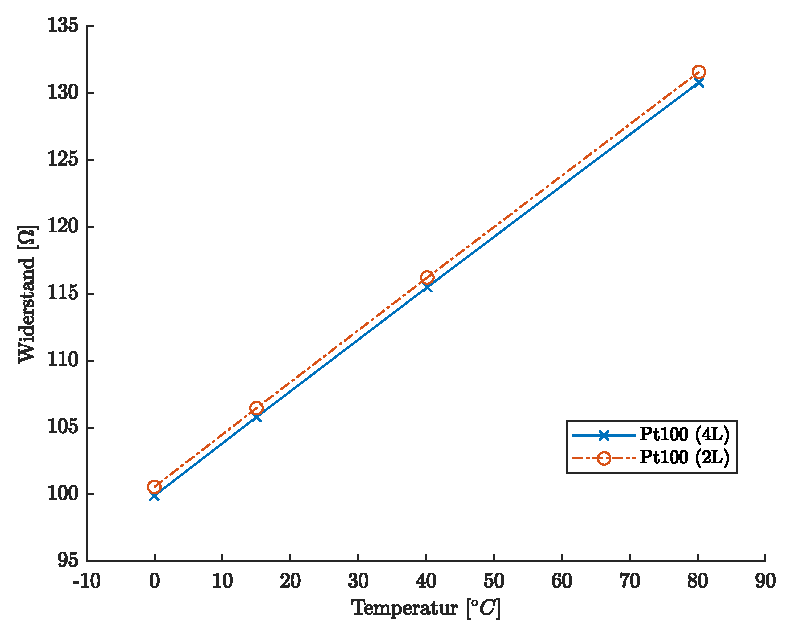
\includegraphics[height=0.3\textheight]{../MLAB/Vergleich2L4L.eps}
	\caption[Temperaturverlauf des Pt100 Temperatursensors mittels Wassertripelpunktzelle]{ Temperaturverlauf des Pt100 Temperatursensors mittels Wassertripelpunktzelle im Metallblockkalibrator.}
	\label{fig:2L4L}
\end{figure}

In folgender Tabelle sind die Differenzen des Pt100 in Zwei und Vierleiter für die Messpunkte aufgetragen.

\begin{table}[H]
	\centering
	\caption{Differenz der Widerstände der Temperatursensoren von Zwei- und Vierleiterschaltung bei den eingestellten Temperaturpunkten und der gewichtete Mittelwert über den Messbereich.}
	\label{tab:VergleichTPZ}
	\begin{tabular}{cccccc}
		Temperatur [\si{\celsius}] & \SI{0}{\celsius} & \SI{20}{\celsius} & \SI{40}{\celsius}&\SI{80}{\celsius} & avg\\ 
		$\Delta$R [\ohm] & \num{0,6582} & \num{0.6688} &  \num{0,7259}& \num{0,7259}& \num{0.7071} \\
	\end{tabular} 
\end{table}

Aus den berechneten Differenzen für die Widerstandswerte lässt sich erkennen, dass der Leitungswiderstand mit steigenden Temperaturen zunimmt. Dieses Verhalten ist nach den physikalischen Gesetzmäßigkeiten zu erwarten. Da das Anschlusskabel nur eine definierte Länge aufweist, wurde für die Abschätzung der Kabellänge der Mittelwert über die Messwerte gebildet und die Kabellänge unter der Annahme der Temperaturunabhängigkeit des Widerstandes berechnet. 

Nach folgender Gleichung \ref{eq:Kabellänge} kann daraus die Länge des Anschlusskabels berechnet werden. Die Angaben für den spezifischen Widerstand der Kabelader und der Kabelquerschnitt wurden den Praktikumsunterlagen entnommen:

\begin{equation}
\label{eq:Kabellänge}
l_{Kabel}= \frac{\Delta R*A_{Quer}}{\rho}=\frac{\SI{0,7071}{\ohm}*\SI{0,1}{\milli\meter\squared}}{\SI{0,0278}{\ohm\milli\meter\squared\per\meter}}=\SI{2,5}{\meter}
\end{equation}

\begin{center}
	\begin{small}
		$l_Kabel$: Länge des Anschlusskabels des Temperatursensors des Pt100,
		$\Delta R$: gemittelte Differenz der Widerstandswerte des Pt100 4L und Pt100 2L,
		$A_{Quer}$: Querschnittfläche des Kabels,
		$\rho$: spezifischer Widerstand einer Ader des Kabels.
	\end{small}
\end{center}

Die berechnete Kabellänge für den Anschluss beträgt \SI{2,5}{\meter}.

\subsubsection{Spannungsverlauf des Thermoelements}

Bei dem Versuch wurde unter Anderem ein Thermoelement vermessen. In der folgenden Abbildung \ref{fig:Spannung} ist der Spannungsverlauf des Thermoelements in Abhängigkeit der Temperatur im Bereich von \SI{0}{\celsius} bis \SI{80}{\celsius} aufgetragen. Es wurde für den Zusammenhang folgende Regressionsfunktion ermittelt:
	
Spannung
Linear model Poly1:
ans(x) = p1*x + p2
Coefficients (with 95% confidence bounds):
p1 =   3.997e-05  (3.847e-05, 4.146e-05)
p2 =   -0.001066  (-0.001134, -0.000998)
[12:56]
sse: 8.9109e-10
rsquare: 0.9998
dfe: 2
adjrsquare: 0.9998
rmse: 2.1108e-05

\begin{figure}[H]
	\centering
	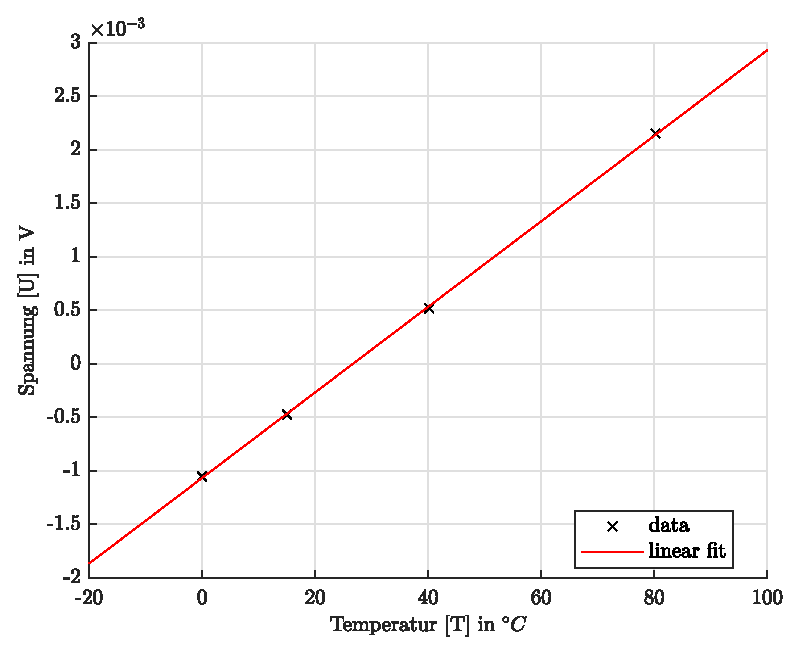
\includegraphics[height=0.3\textheight]{../MLAB/Spannung.eps}
	\caption[Spannungverlauf des Thermoelements in Abhängigkeit der Temperatur im Bereich von \SI{0}{\celsius} bis \SI{80}{\celsius} ]{Spannungverlauf des Thermoelements in Abhängigkeit der Temperatur im Bereich von \SI{0}{\celsius} bis \SI{80}{\celsius}.}
	\label{fig:Spannung}
\end{figure}

\subsubsection{Anwendungsgebiete verschiedener Sensoren}

Die verschiedenen Temperatursensoren finden im Alltag und der Technik verschiedenste Anwendungsfelder und decken damit individuell optimal verschiedenste Anforderungen ab. 

NTC zeichnen sich durch ihren negativen Temperaturkoeffizienten aus. Ihr Widerstand sinkt bei steigender Temperatur ab. Sie finden häuftig Anwendung in der Medizintechnik, beispielsweise in Dialysegeräten, DNA-Sequenzierern und Blutanalysegeräten und könen auch noch optimal in Temperaturbereichen bis \SI{-150}{\celsius} betrieben werden. Sie finden zusätzlich Anwendung in Küchenherden oder Haushaltsgeräten oder bei der Regelung von Akkutemperaturen für Elektroautos. 

Thermoelemente zeichnen sich in der Anwendung bei extremen Temperaturen und Umweltbedingungen aus. Sie können häufig Temperaturen von bis zu \SI{1700}{\celsius} betrieben werden. 

Platin-Temperatursensoren zeichnen sich durch ihren linearen Widerstand über einen großen Temperaturbereich aus (\SI{-200}{\celsius} bis \SI{1000}{\celsius}), was eine sehr stabile Temperaturmessung über sehr große Messbereiche ermöglicht. Sie finden häufig Anwendung in Lebensmittelverarbeitungsanlagen, in der Raumfahrt oder zur Messung von Abgastemperaturen in der Automobilindustrie. Platin ist quasi chemisch inert, sodass es selbst bei Feuchte, korrosiver Umgebung und weiteren extremeren Umweltbelastungen zuverlässig funktionieren kann. 

In großen Fertigungsanlagen war es früher üblich kostengünstigere Thermometer in Zweileiter-Schaltung anzuschließen. Die durch den Leitungswiderstand entstehende Messfehler wurden tabellarisch aufgeführt und die systematischen Fehler mithilfe der Korrektur-Tabellen angepasst. Mit heutiger digitaler Technik können diese Werte direkt bei der Messung voreingestellt und automatisch korrigiert werden. 

\subsection{Teil II: Identifizierung der Sensoren}

Für die Identifizierung der Temperatursensoren unterschiedlicher Typen stand ein Multimeter und die Kennliniendiagramme verschiedener Widerstandssensoren aus dem Praktikumsskript zur Verfügung. Die verschiedenen Temperatursensoren wurden jeweils an das Multimeter angeschlossen und ihr Widerstand bei Raumtemperatur (ca. \SI{23}{\celsius}) ermittelt. Anschließend wurde der jeweilige Sensor mit der Hand erwärmt, was zu einem Temperaturanstieg und der Veränderung des Widerstands führte. Anhand der erhaltenen Widerstandswerte wurde mithilfe der Kennliniendiagramme der jeweilige Sensor identifiziert. 
Folgende Sensoren wurden anhand dieser Methode identifiziert:

Sensor 1: NTC\\
Sensor 2: Thermoelement\\
Sensor 3: Pt 1000\\
Sensor 4: KTY\\
Sensor 5: Pt100 2L\\
Sensor 6: Pt100 4L\\

\subsection{Teil III: Wärmebildkamera}

Für den Versuch Wärmebildkamera wurde die verschiedenen Probenplatten (s. Abb. \ref{fig:VersuchsaufbauWBK}) in dem temperierten Wasserbad mit der Einstellung von \SI{60}{\celsius} mittels einer Wärmebildkamera des Typs E60 der Firma FLIR verwendet. Für die Wärmebildkamera muss vor der Messung ein Emissgrad eingestellt werden. Hierfür wurde ein Emissionsgrad von $\epsilon=0,95$ gewählt. Die Wärmebildkamera kann bei korrekter Benutzung die Temperatur auf eine Genauigkeit von $\Delta_T = \pm \SI{2}{\celsius}$ ermitteln.

Die rechte Abbildung zeigt beispielhaft ein Foto der Wärmebildkamera mit allen Probenmaterialien. 

\begin{figure}[H]
	\begin{minipage}{0.5\textwidth}
		\centering
		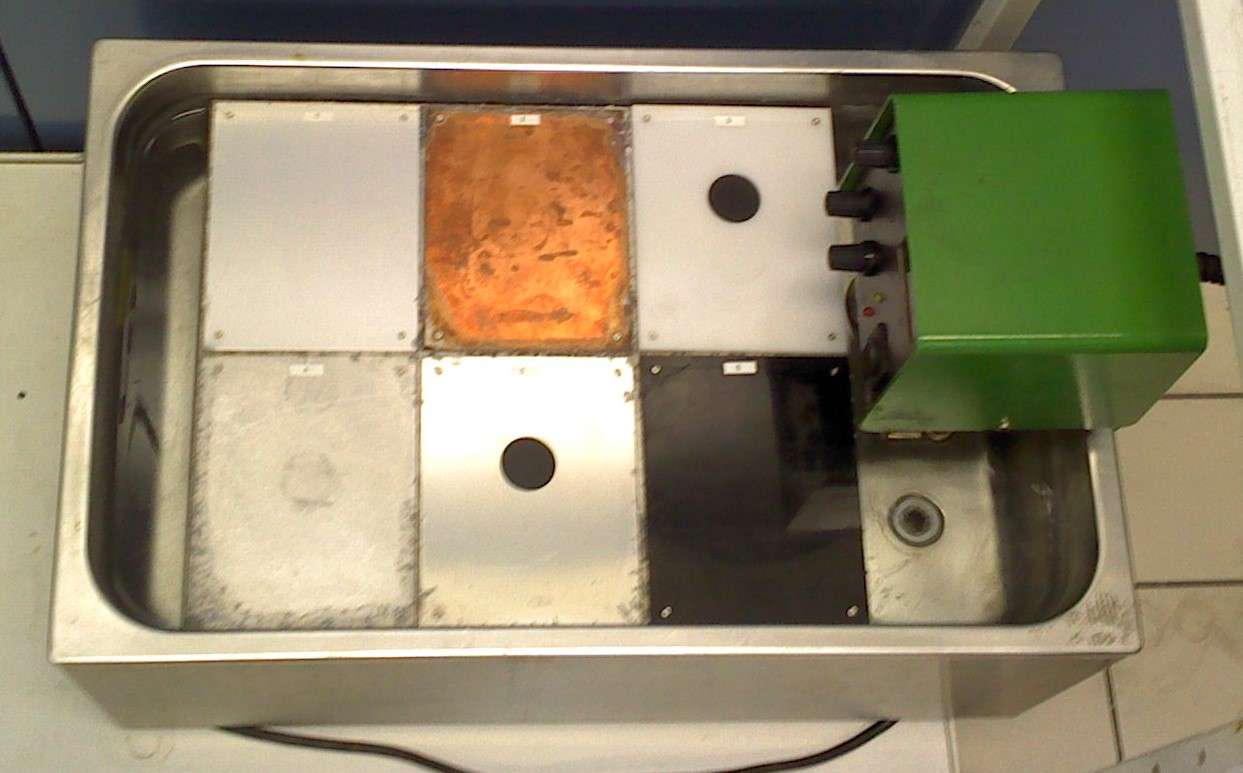
\includegraphics[width=0.8\textwidth]{../FLIR_100/FLIR2240.jpg}
		\caption[Versuchsaufbau Wärmebildkamera]{Versuchsaufbau Wärmebildkamera: Die unterschiedlichen Probenplatten wurden im selben Wärmebad mit \SI{60,0}{\celsius} temperiert.}
		\label{fig:VersuchsaufbauWBK}
	\end{minipage}\hfill
	\begin{minipage}{0.5\textwidth}
		\centering
		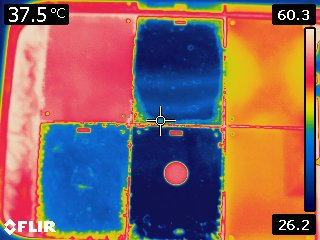
\includegraphics[width=0.6\textwidth]{../FLIR_100/FLIR2241.jpg}
		\caption[Foto der Wärmebildkamera über alle Probenplatten]{Foto der Wärmebildkamera über alle Probenplatten bei gleicher Temperatur.}
		\label{fig:VersuchsaufbauWBK}
	\end{minipage}
\end{figure}

In der folgende Tabelle sind die Probenmaterialien und die mithilfe der Wärmebildkamera und dem Temperaturfühler ermittelten Temperaturen aufgeführt. 

\begin{table}[H]
	\centering
	\caption{Verwendete Probenmaterialien und ermittelte Temperatur durch Wärmebildkamera und Temperaturfühler.}
	\label{tab:Proben,Eigenschaften}
	\begin{tabular}{cccccc}
		Nr. & Bezeichnung & Gruppe & Messpunkt & $T_{WBK} [\celsius]$ & $T_{Fühler} [\celsius]$\\
		\hline
	1& Alu. silber eloxiert&Metall&Nein&57,5&55,6\\
	2& Kupfer glänzend&Metall&Nein&27,8&56,9\\
	3&POM weiß&Kunststoff&Ja&54,5&50,3/50,8\\
	4&Alu. rau&Metall& Nein&32,0&56,4\\
	5&Alu. glänzend& Metall&Ja&27,5/58,0&57,2/56,9\\
	6&POM schwarz&Kunststoff&Nein&53,7&51,5\\	
	\end{tabular} 
\end{table}

Es wurden folgende Beobachtungen gemacht:

- Mit einem für die Wärmebildkamera voreingestellten Emissionsgrad von $\epsilon=0,95$ können die Temperaturen der  Kunststoffe (3 und 6) und des eloxierten (beschichteten) Aluminium (1) annähernd gut ermittelt werden. Da der Emissionsgrad $\epsilon$ der Metalle geringer ist, erscheinen sie in Betrachtung durch die  Wärmebildkamera kälter. \\
- Der aufgeklebte Kunststoffpunkt auf den Proben 3 (weißer Kunststoffpunkt auf Kunststoff) und 5 (schwarzer Kunststoffpunkt auf Metall) ist unabhängig seiner Farbe gut zu erkennen, da sein Emissionsgrad annähernd dem voreingestellten der Kamera entspricht und die Temperatur am aufgeklebten Punkt relativ genau ermittelt werden kann. Der Emissionsgrad ist demzufolge material- aber nicht farbunabhängig. Diese Beobachtung deckt sich zusätzlich mit der direkten Messung der aus dem selben Material bestehenden Kunststoffproben unterschiedlicher Farbe (3 und 6). \\
-  Steht die Kamera korrekt (senkrecht, ca. \SI{1}{m} über dem Messobjekt) können sich teilweise die Wärmeabstrahlung der Deckenbeleuchtung oder Wärmeabstrahlung von beispielsweise Händen die senkrecht über die Kamera gehalten werden von dieser zusätzlich durch Reflexion an beispielsweise den Metallproben erfasst werden, sodass das Messobjekt mit einer Schattenabbildung der Lampe oder der Hand fotografiert wird. \\
- Wird der Winkel oder die Entfernung der Wärmebildkamera zum Messobjekt verändert, kann diese die Temperatur nicht mehr optimal ermitteln. Durch Spiegelungen und Reflexionen erscheinen die Materialien teilweise wärmer oder kälter, auch innerhalb einer Materialprobe. 

\begin{figure}[H]
	\begin{minipage}{0.5\textwidth}
		\centering
		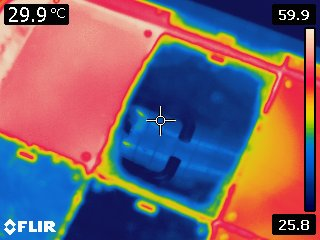
\includegraphics[width=0.8\textwidth]{../FLIR_100/FLIR2249.jpg}
		\caption[Ermitteltes Wärmekamerafoto mit Hand als Störfaktor]{Ermitteltes Wärmekamerafoto mit Hand als Störfaktor.}
		\label{fig:WBKHand}
	\end{minipage}\hfill
	\begin{minipage}{0.5\textwidth}
		\centering
		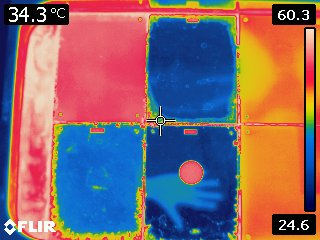
\includegraphics[width=0.8\textwidth]{../FLIR_100/FLIR2243.jpg}
		\caption[Ermitteltes Wärmekamerafoto mit Deckenbeleuchtung als Störfaktor]{Ermitteltes Wärmekamerafoto mit Deckenbeleuchtung als Störfaktor}
		\label{fig:WBKDecke}
	\end{minipage}
\end{figure}

\subsubsection{Berechnung der Emissionsgrade}

Die mit dem Messfühler ermittelte Temperatur der Proben wird im folgenden als die wahre Temperatur angenommen. Über die mit der Wärmebildkamera ermittelte Temperatur und der Angabe der Umgebungstemperatur, kann über folgende Formel der Emissionsgrad des jeweiligen Materials bestimmt werden. 

KACKFormel umstellen!!!!
und Emissionsgrade berechnen! 
\newpage
\section{Anhang}

\subsection{Teil I: Kalibrierung}

\subsubsection{Fixpunktkalibration an der Wassertripelpunktzelle}

In der folgenden Abbildung \ref{fig:Fixpunkt} wird der Temperaturverlauf in Abhängigkeit der Zeit (die Scanrate beträgt \SI{1}{\second}) für den Pt-100 Sensor abgebildet. 

\begin{figure}[H]
	\centering
	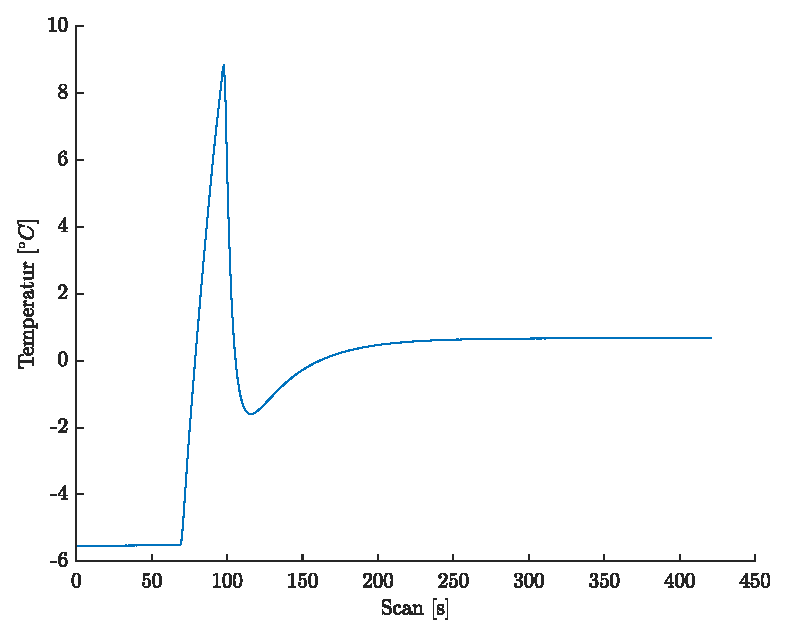
\includegraphics[height=0.2\textheight]{../MLAB/Fixpunktkalibration.eps}
	\caption[Temperaturverlauf des Pt100 Temperatursensors mittels Wassertripelpunktzelle]{ Temperaturverlauf des Pt100 Temperatursensors mittels Wassertripelpunktzelle im Metallblockkalibrator.}
	\label{fig:Fixpunkt}
\end{figure}

\subsection{Teil III: Wärmebildkamera}

Aufgenommene Bilder des Versuchsstandes und Bilder der Wärmebildkamera. 
Die rechte Abbildung zeigt beispielhaft ein Foto der Wärmebildkamera mit allen Probenmaterialien. 

\begin{figure}[H]
		\centering
		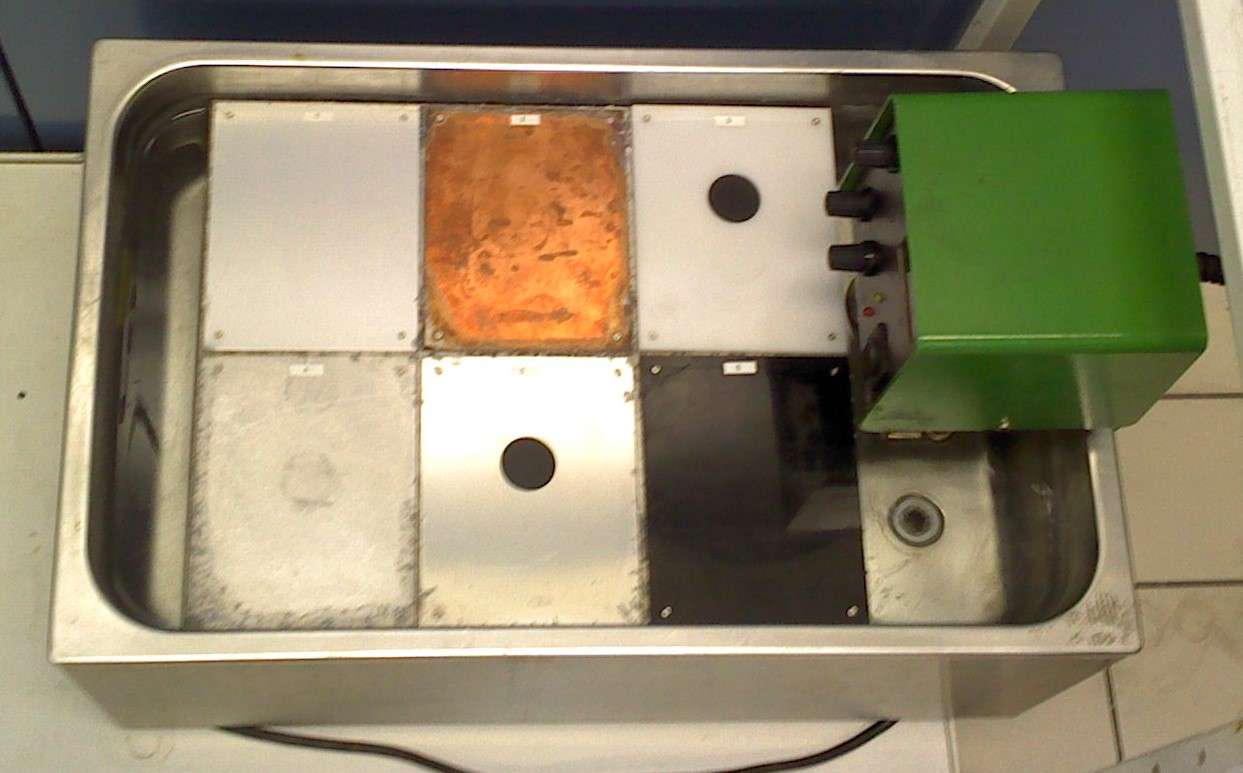
\includegraphics[width=0.5\textwidth]{../FLIR_100/FLIR2240.jpg}
		\caption{Versuchsaufbau Wärmebildkamera: Die unterschiedlichen Probenplatten wurden im selben Wärmebad mit \SI{60,0}{\celsius} temperiert.}
		\label{fig:VersuchsaufbauWBK}
\end{figure}

\begin{figure}[H]
		\centering
		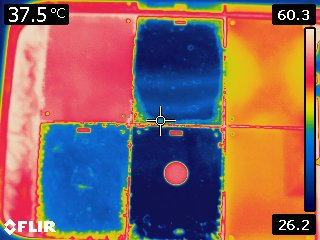
\includegraphics[width=0.4\textwidth]{../FLIR_100/FLIR2241.jpg}
		\caption{Foto der Wärmebildkamera über alle Probenplatten bei gleicher Temperatur.}
		\label{fig:FotoWBK}
\end{figure}

\begin{figure}[H]
		\centering
		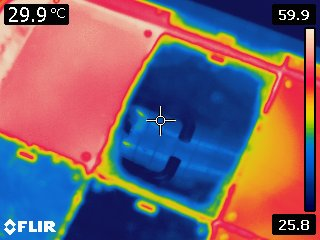
\includegraphics[width=0.4\textwidth]{../FLIR_100/FLIR2249.jpg}
		\caption[Ermitteltes Wärmekamerafoto mit Hand als Störfaktor]{Ermitteltes Wärmekamerafoto mit Hand als Störfaktor.}
		\label{fig:WBKHand}
\end{figure}

\begin{figure}[H]
		\centering
		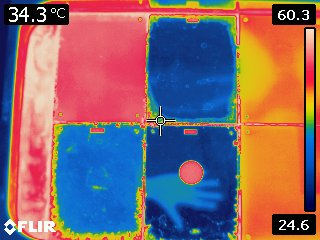
\includegraphics[width=0.4\textwidth]{../FLIR_100/FLIR2243.jpg}
		\caption[Ermitteltes Wärmekamerafoto mit Deckenbeleuchtung als Störfaktor]{Ermitteltes Wärmekamerafoto mit Deckenbeleuchtung als Störfaktor}
		\label{fig:WBKDecke}
\end{figure}

%\newpage
%\input{sections/04_Zusammenfassung_und_Ausblick}

%\newpage
%\printbibliography


\end{document}